\documentclass[../main.tex]{subfiles}
\graphicspath{{\subfix{../images/}}}
\begin{document}

\noindent
\begin{tabular}{p{6cm}p{5.9cm}}
  {Stand\label{Ex:CentralAxis}\index{exercise!central axis} up} straight and close your eyes.
Imagine a {stream of energy} flowing between your feet upwards, through your body (central axis).
Feel how your skeleton, how your musculature and their tissues and the organs {organize themselves around this central axis}.
Everything is in movement.
Take your time, allow changes to happen even to the organisation on a cellular level.

Start {turning} around the axis with little steps, one way, then the other.
{Repeat this}.
Then stop and {orient yourself} in this position, correct yourself if necessary.
Feel again the sensation of this central axis.

You may add this exercise to your {morning program},
or practice it when you feel that you fell out of your {center}.
  Enjoy this feeling of the central axis and take it into your everyday life. &
  \raisebox{-\totalheight}{  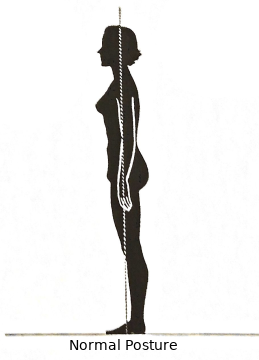
\includegraphics[width=5.9cm]{Normal_Posture} } \\

\end{tabular}

{Actively registering} what you feel accelerates your progress.
It happens completely from your {feelings} and there's no need for perfection.
Your new {perception of your body} will stay more present this way and you will be able to {build on it} as a foundation.
Give your body the time needed, be {affectionate} with it and celebrate every progress.
\end{document}